\chapter{Redmine}\label{chp:redmine}

\section{Introdução}\label{sec:redmine-introducao}
Neste capítulo vamos explicar como o Redmine, uma ferramenta de gerenciamento de projetos foi utilizada para gestão de processos, ilustrando com um exemplo. Vamos apresentar ainda, a capacidade extensiva desta ferramenta através do desenvolvimento de \textit{plugins}. Por último vamos abordar as limitações do Redmine que nos motivaram a desenvolver algo novo para atingir nosso objetivo em automatização de processos.

O Redmine\cite{redmine} é uma ferramenta \textit{open-source} de gerenciamento de projetos. Foi criada por Jean-Philippe Lang em 2006. Desenvolvido em \textit{Ruby}, utilizando a \textit{framework} \textit{Rails}, tem como objetivo dar flexibilidade de configuração ao usuário, e também ao desenvolvedor.


\section{Estrutura básica do Redmine}\label{sec:redmine-estrutura_basica}

A estrutura básica de gerenciamento de projetos no Redmine é composta por 6 principais elementos. São eles:

\subsection{Projetos}\label{subsection:redmine-estrutura_basica-projeto}

Projetos são o objeto central do Redmine. Eles são compostos por diversos módulos que acrescentam diferentes dimensões para o seu gerenciamento, como gerenciamento de tarefas, planejamento de etapas e marcos no projeto, acompanhamento do progresso das tarefas em um diagrama de \textit{Gantt}, \textit{Wiki} para organização do conhecimento, entre outros. 
\subsection{Tarefas}\label{subsection:redmine-estrutura_basica-tarefa}

São as unidades básicas de execução de trabalho dos projetos (\ref{subsection:redmine-estrutura_basica-projeto}). Elas contém os dados relevantes para o seu gerenciamento (e.g, tipo (\ref{subsection:redmine-estrutura_basica-tracker}), situação (\ref{subsection:redmine-estrutura_basica-status})), para a sua execução (e.g, título, descrição) e dados adicionais que podem variar entre os projetos e tipos de tarefa, que são cadastrados como campos personalizados (\ref{subsection:redmine-estrutura_basica-custom_fields}).  


\subsection{Tipos de tarefa}\label{subsection:redmine-estrutura_basica-tracker}

Tipos de tarefa definem o fluxo de trabalho para a realização de atividades similares. De acordo com o tipo, variam as informações necessárias para a execução da tarefa, a sequência de passos para sua conclusão e as ações que cada membro do projeto pode desempenhar em cada etapa.

\subsection{Situação das tarefas}\label{subsection:redmine-estrutura_basica-status}

Situação indica em qual etapa do processo uma tarefa se encontra. Na tela de fluxo de trabalho, é possível configurar, para cada papel, tipo de tarefa e situação, quais campos do formulário podem ser visualizados, ou editados.

\subsection{Papéis de usuários}\label{subsection:redmine-estrutura_basica-role}

Os papéis de usuários definem quais permissões um usuário possui, como, por exemplo, visualizar, adicionar e editar tarefas, editar \textit{Wiki}, adicionar e editar documentos. Os papéis são atribuídos aos usuários em cada projeto que ele participa, portanto, ele pode possuir permissões diferentes dependendo do projeto de que ele é membro.

\subsection{Campos Personalizados}\label{subsection:redmine-estrutura_basica-custom_fields}

Todas as tarefas de projetos possuem dados em comum, como data de início, data de término e descrição. No entanto, dependendo das especificidades de um projeto ou tipo de tarefa, podem ser necessárias informações adicionais. Para esses casos existem os campos personalizados. Eles permitem criar novos campos e adicioná-los às tarefas, estendendo as configurações padrão da ferramenta.

\section{Gestão de processos com o Redmine}\label{sec:redmine-gestao_processos}

A estrutura de projetos do Redmine é altamente configurável. Todos os elementos explicados na seção \ref{sec:redmine-estrutura_basica} são cadastrados pelos usuários administradores do sistema, que são responsáveis por configurá-los e personalizá-los para atender às demandas de cada projeto.

Todas as configurações e personalizações citadas no último parágrafo são feitas exclusivamente pela interface da ferramenta, sem necessidade de alterações no código da aplicação ou arquivos de configuração, o que confere aos administradores capacidade para modelar a estrutura da ferramenta da forma que for mais conveniente para a necessidade dos usuários.

Além disso, o módulo de gerenciamento de tarefas permite ao usuário interagir muito bem com o projeto, tendo total controle de suas tarefas, e ainda submetido a um controle de acesso bem detalhado e flexível.

As vantagens citadas acima, e ainda o fato de o Redmine ser \textit{open-source}, com uma grande comunidade de usuários e desenvolvedores foram motivadoras para a utilização deste como um gerenciador de processos.

\section{Modelando processos com o Redmine}\label{sec:redmine-automatizar_processo}

O primeiro passo para modelar um processo é identificar como representá-lo na estrutura do Redmine.

Nesta seção descreveremos como utilizar o potencial de configuração do Redmine para utilizá-lo fora do contexto de gerenciamento de projetos e aplicá-lo como ferramenta de automatização de processos. Explicaremos, também, como definir os atores de um processo, as ações permitidas a cada um deles, especificar os fluxos de trabalho e como gerenciar os dados relevantes ao seu contexto. Estes passos serão ilustrados na implementação do caso de uso descrito na seção \ref{sec:problema-exemplo}.


\subsection{Modelando processos}\label{subsection:redmine-automatizar_processo-criacao}

Ao configurar um tipo de tarefa, definimos as etapas de um processo, representadas pelas situações (\ref{subsection:redmine-estrutura_basica-status}) e quais campos (\ref{subsection:redmine-estrutura_basica-custom_fields}) são utilizados para guardar informações relativas à execução de um processo.

Durante a criação do tipo de tarefa são definidas qual situação (\ref{subsection:redmine-estrutura_basica-status}) é a padrão para aquele tipo, em quais projetos ele é utilizado e quais campos (\ref{subsection:redmine-estrutura_basica-custom_fields}) ele utiliza para guardar informações.


\subsection{Definição dos atores}\label{subsection:redmine-automatizar_processo-atores}

\subsubsection{Escolha dos atores}

Os atores de um processo são definidos nos projetos que o tipo de tarefa está relacionado. Ao associar um papel a um usuário (ou grupo de usuários) é definido quais papéis ele terá naquele projeto - no caso de um grupo de usuários ser associado a um projeto, todos os seus membros herdarão os papéis atribuídos a ele.

\subsubsection{Definição das permissões dos atores}

As permissões dos atores do processo são definidas nos papéis de usuários (\ref{subsection:redmine-estrutura_basica-role}). Neles é possível escolher se um usuário pode ter tarefas atribuídas a ele, quais tarefas ele consegue visualizar e quais ações ele é capaz de realizar sobre as tarefas (e.g. Ver Chamados, Editar Chamados, Adicionar Chamados, Adicionar Notas).

\subsection{Fluxo de trabalho}

A configuração do fluxo de trabalho é onde se orquestra o processo e define-se como os usuários podem manipular os dados dos chamados. Essa configuração é divida em duas partes, permissão de campos e transição de estados, e é feita separadamente para cada papel.

As permissões de campos ditam de que forma um usuário pode interagir com os campos dos chamados que pode editar dependendo da situação atual do chamado. Baseado nessas permissões um campo pode ficar disponível somente para leitura, editável, ou obrigatório. A figura \ref{fig:redmine_campos} apresenta a tela de configuração de permissão dos campos no Redmine.

\begin{figure}[H]
  \centering
  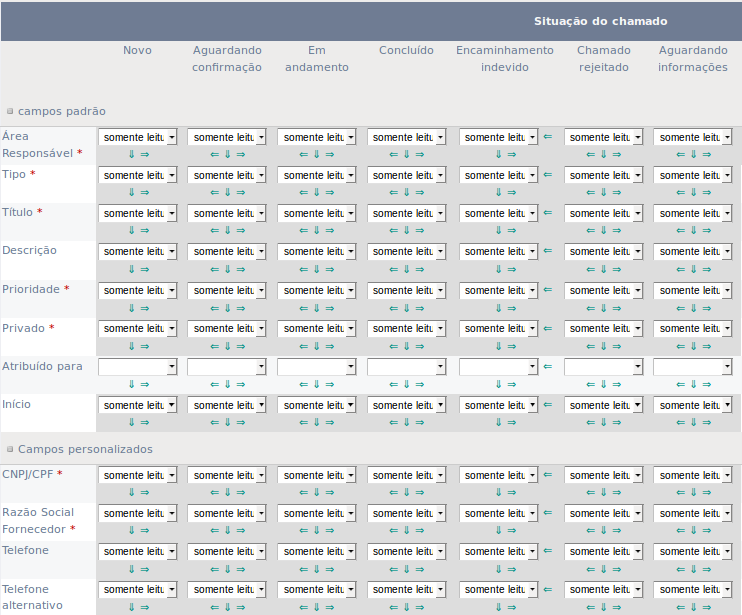
\includegraphics[width=1.0\textwidth]{imagens/workflow_fields.png}
  \caption{Tela de configuração de permissão de campos do fluxo de trabalho}
  \label{fig:redmine_campos}
\end{figure}

A transição de estados define para quais situações um chamado pode ser alterado de acordo com o estado atual, determinando para quais etapas de um processo um usuário consegue conduzir a tarefa. A figura \ref{fig:redmine_transicoes} apresenta a tela de configuração das transições de estados no Redmine.

\begin{figure}[H]
  \centering
  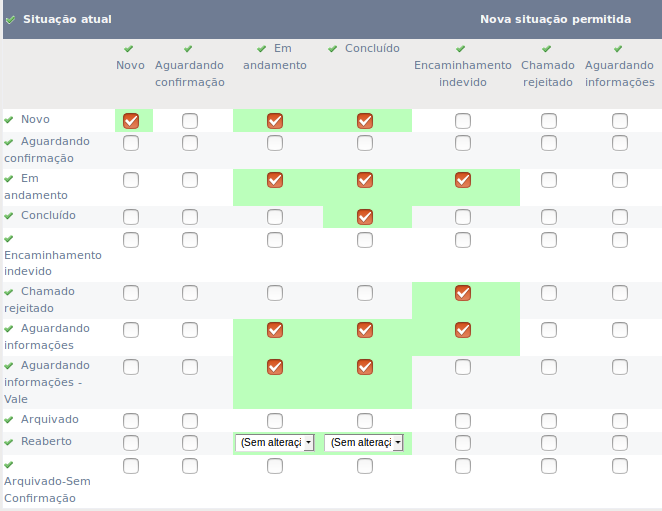
\includegraphics[width=1.0\textwidth]{imagens/workflow_status.png}
  \caption{Tela de configuração das transições de situação do fluxo de trabalho}
  \label{fig:redmine_transicoes}
\end{figure}

\section{Precificação manual}\label{sec:redmine-impl-caso-uso}

Para implementar o caso de uso foi criado um tipo de tarefa chamado Precificação manual. Também foram criadas as situações Novo, Solicitar troca de preço, Aguardando aprovação, Não aprovado, Trocar preço, Encerrado.

As situações acima representam cada etapa do processo, que na modelagem em BPMN são caixinhas. A transição de situação é feita pelo responsável pela tarefa naquele momento, que também altera para o novo responsável na próxima etapa, caso necessário. A etapa de troca de preço consiste da operação de um sistema externo, e assim que concluída, o responsável conclui o processo, passando-o para a próxima etapa.

Esta implementação mostra como processos simples podem ser modelados no Redmine desta forma, se aproveitando de toda a sua estrutura de tarefas. Desta forma é possível que um usuário acompanhe processos, execute etapas manuais no processo, preenchendo formulários, e tomando decisões as próximas etapas, como a etapa de aprovação.

A ferramenta escolhida se mostrou uma solução barata, de rápida implementação, e que permite que o próprio usuário administrador fique responsável pela manutenção. Muitos cenários problemáticos, como apresentado no capítulo anterior, são simples, e para que rodem melhor precisam de uma padronização e automação mínima, que a utilização do Redmine pode oferecer, e transformar o quadro de uma área inteira de um negócio.

\section{Cenário com aprovação paralela}\label{sec:cenario-complexo}

Apesar do grande potencial de configuração do Redmine e de suportar a automatização de processos simples, não é possível utilizá-lo em situações de maior complexidade. A modelagem de processos neste sistema é baseada em uma máquina de estados cujas transições são definidas apenas pelo estado atual do processo e do perfil de acesso dos usuários. Portanto, fluxos mais complexos que possuem, por exemplo, atividades executadas em paralelo ou regras de negócio dependentes de variáveis do contexto de cada execução de um processo não são possíveis de ser modelados apenas com as configurações padrão do Redmine.

Digamos que o processo descrito na figura \ref{fig:exemplo_bpmn} se tornasse um pouco mais complexo, e a troca de preço precisasse ser aprovada por 3 gestores em paralelo, e a reprovação de qualquer um deles reprovasse a precificação. Este caso já não é suportado pelo Redmine. No entanto, este sistema foi desenvolvido de forma a permitir a criação de funcionalidades complementares.

O Redmine foi desenvolvido de forma a ser extensível por meio de \textit{plugins}. Uma funcionalidade da ferramenta pode ser modificada, ou uma nova funcionalidade criada sem precisar alterar o código original do Redmine. Os \textit{plugins} são desenvolvidos em \textit{Rails}, o mesmo \textit{framework} de programação do Redmine. 

Para possibilitar extensões de funcionalidades que envolvem enxertar pedaços de código no meio de uma classe ou de uma tela, o Redmine disponibiliza \textit{hooks} em diversas partes da ferramenta. São \textit{tags} com um identificador da parte do código em que estão inseridas. E para utilizar este \textit{hook} basta incluir um \textit{hook} \textit{listener} num \textit{plugin}, e direcionar qual arquivo ou método um determinado \textit{hook} vai disparar.

Muitos plugins desenvolvidos pela comunidade estão disponíveis e podem ser usado para aumentar o poder de modelagem de processos, tornando o Redmine uma ferramenta ainda mais flexível. Esta facilidade abre as portas para estender o Redmine para possibilitar a implementação de processos mais complexos.  